\documentclass[a4paper, 11pt]{article}
\usepackage[utf8]{inputenc}
\usepackage{amsmath}
\usepackage{array}
\usepackage{amssymb} 
\usepackage{array,multirow,makecell}
\usepackage{comment}
\usepackage{fullpage} 
\usepackage{graphicx}
\usepackage{bussproofs}
\usepackage{mathtools}
\graphicspath{ {./images/} }

\usepackage{tcolorbox}
\usepackage{listings}
\usepackage{xcolor}

\definecolor{codegreen}{rgb}{0,0.6,0}
\definecolor{codegray}{rgb}{0.5,0.5,0.5}
\definecolor{codepurple}{rgb}{0.58,0,0.82}
\definecolor{backcolour}{rgb}{0.95,0.95,0.92}
 
\lstdefinestyle{mystyle}{
    backgroundcolor=\color{backcolour},   
    commentstyle=\color{codegreen},
    keywordstyle=\color{magenta},
    numberstyle=\tiny\color{codegray},
    stringstyle=\color{codepurple},
    basicstyle=\ttfamily\footnotesize,
    breakatwhitespace=false,         
    breaklines=true,                 
    captionpos=b,                    
    keepspaces=true,                 
    numbers=left,                    
    numbersep=5pt,                  
    showspaces=false,                
    showstringspaces=false,
    showtabs=false,                  
    tabsize=2
}
 
\lstset{style=mystyle}

\newtcolorbox{mybox}[3][]
{
  colframe = #2!25,
  colback  = #2!10,
  coltitle = #2!20!black,  
  title    = {#3},
  #1,
}

\title{Logique 1A}

\begin{document}

\maketitle

\section{Introduction}

En logique du premier ordre et, en particulier, en théorie de la démonstration, les objets que l'on étudie sont les \textit{formules} et leur \textit{démonstrations}. Les termes et les formules forment la grammaire d'une langue, simplifiée à l'extrême et calculée exactement pour dire ce que l'on veut sans ambiguïté et sans détour inutiles.

\

\underline{\textit{Les termes.}} Ils distinguent les objets dont on veut prouver les propriétés.

\underline{\textit{Les formules.}} Elles représentent les propriétés des objets que l'on étudie.

\underline{\textit{Les démonstrations.}} Elles permettent d'établir qu'une formule est \textit{vraie}.

\subsection{Les formules}

\subsubsection{Le langage}

En mathématiques, on utilise, suivant le domaine, différents langages qui se distinguent par les symboles utilisés. La définition ci-dessous exprime simplement qu'il suffit de donner la liste de ces symboles pour préciser le langage.

\

\begin{tcolorbox}
    \textbf{Définition:} Un \textit{langage} est la donnée d'une famille (pas nécessairement finie) de symboles. On en distingue trois sortes:
    
    \begin{itemize}
        \item les symboles de \textit{constante};
        \item les symboles de \textit{fonction}. A chaque symbole est associé un entier strictement positif qu'on appelle son \textit{arité}: c'est le nombre d'arguments de la fonction. Si l'arité est 1 (resp. 2, ..., $n$), on dit que la fonction est \textit{unaire} (resp. \textit{binaire}, ... \textit{$n$-aire})
        \item les symboles de \textit{relation}. De la même manière, à chaque symbole est associé un entier positif ou nul (son arité) qui corréspond au nombre d'arguments et on parle de relation \textit{unaire, binaire, $n$-aire.}
    \end{itemize}
    
\end{tcolorbox}

\

\noindent
\underline{Exemple:} \\

    Le langage de l'analyse réelle continent les symboles:
    
    \begin{itemize}
        \item constantes: $0, 1, ..., e, ..., \pi$
        \item fonctions: $+, -, |.|, \sin, \ln, ...$
        \item relations: $=, \geq, \leq, ...$
    \end{itemize}

\subsubsection{Les termes}

On se donne un ensemble (infini) $V$ de variables. Les variables seront notées: $x, y, z, ...$ (éventuellement indexées: $x_1,..$)

\

Les \textit{termes} (ou \textit{termes du premier ordre}) représentent les objets associés au langage. \\ Formellement:

\

\begin{tcolorbox}
    \textbf{Définition:} Soit $L$ un langage et $(T_i)_{i \in \mathbb{N}}$ une famille d'ensembles.
    
    \
    
    L'ensemble $T$ des termes est $T = \bigcup_{k \in \mathbb{N}} T_{k}$ où:
    \begin{itemize}
        \item $T_0 = \{ t / t$ est une variable ou un symbole de constante\}
        \item $\forall k \in \mathbb{N}^*, T_{k+1} = T_k \cup \{f(t_1, ..., t_n) / t_i \in T_k$ et $f$ le symbole de fonction d'arité $n$\}
    \end{itemize}
    
On appellera \textit{hauteur} d'un terme $t$ le plus petit $k$ tel que $t \in T_k$.

Un terme \textit{clos} est un terme qui ne contient pas de variables.
    
\end{tcolorbox}

Cette définition ne fait que donner des règles d'écriture. Il faut donc la comprendre sous la forme: si $f$ est un symbole, on peut \textit{écrire} $f(t_1, ..., t_n)$. Le choix de cette écriture n'est pas neutre puisque son \textit{sens} est l'application d'une fonction à ses arguments.

\

\noindent
\underline{Exemple:} 

Sur le langage précédent, $\sin(\ln(x)+\cos(|y + e|))$ est un terme et $\ln(|\cos(e) - \sin(e)|)$ est un terme clos.

\

\noindent
\underline{Remarque:} 

Il est souvent commode de voir un terme comme un arbre dont chaque noeud est étiqueté par un symbole de fonction et chaque feuille par une variable ou une constante. Par exemple, le terme $(x+2).\sin(y + \ln(x))$ est représenté par l'arbre suivant:

\begin{center}
    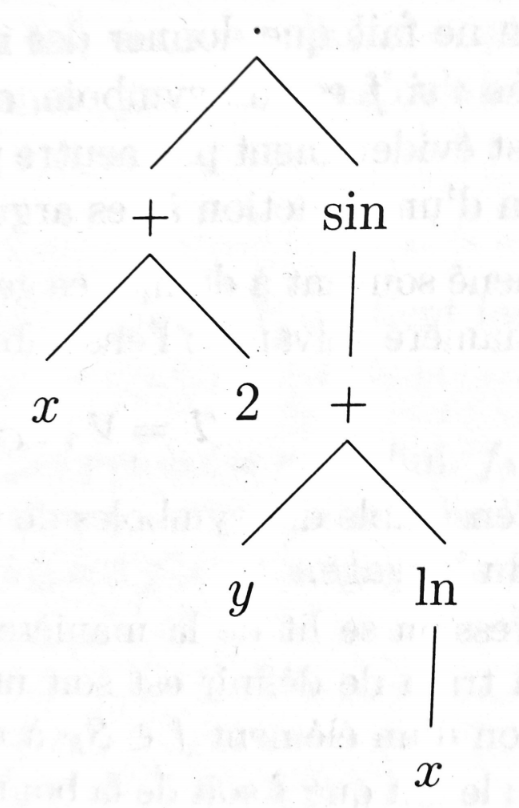
\includegraphics[scale = 0.2]{./1.png}
\end{center}

\

Pour prouver une propriété $P$ sur les termes, il suffit de prouver $P$ pour les variables et les constantes et de prouver $P(f(t_1, ..., t_n))$ à partir de $P(t_1, ..., t_n)$. On fait une preuve par induction sur la hauteur d'un terme.

\

Pour définir une fonction $\phi$ sur les termes, il suffit de la définir sur les variables et les constantes et de dire comment on obtient $\phi(f(t_1, ..., t_n))$ à partir de $\phi(t_1), ..., \phi(t_n)$. On fait ici une définition par induction sur la hauteur d'un terme.

\

Ainsi, avant d'avancer, il faut rappeler ce qu'est l'induction.

\section{L'Induction}

\subsection{Rappel sur les prédicats}

\begin{tcolorbox}
    \textbf{Définition:} Un prédicat est une fonction dont la valeur est vrai ($\top$) ou faux ($\bot)$. 
\end{tcolorbox}

Une famille de prédicats est par exemple l'ensemble des prédicats sur ls entiers, c'est à dire les fonctions de la forme:

\begin{equation*}
    P: \mathbb{N} \rightarrow \{\top, \bot\}
\end{equation*}

Exemple:

\

Soit $P: \mathbb{N} \rightarrow \{\top,\bot\}$ le prédicat défini par:

\begin{equation*}
    P(n) = 
    \begin{cases*}
      \top & \text{si $\sum_{i=0}^{n} 2^i = 2^{n+1} - 1$} \\
      \bot & \text{sinon}
    \end{cases*}
\end{equation*}

\subsubsection{L'induction mathématique}

Dans l'exemple précédent, on peut démontrer que le prédicat $P(n)$ est vrai pour tout $n \geq 0$. Ainsi, les assertions $P(0), P(1), P(2), P(3), P(4), ... $ sont vraies. Mais comment peut-on prouver qu'une infinité d'assertions sont vraies ?

\

\textbf{Première stratégie naïve:}

1. On commence par prouver que $P(1)$ est vrai.

2. On montre ensuite que $P(1) \Rightarrow P(2)$ est vrai.

3. On utilise le modus ponens pour en déduire que $P(2)$ est vrai.

4. On montre que $P(2) \Rightarrow P(3)$ est vrai.

5. On utilise le modus ponens pour en déduire que $P(3)$ est vrai. ECT...

\

Le problème de l'infinité d'étapes pour montrer que $P(n)$ est vrai pour tout $n \geq 0$ n'est pas encore reglé, mais il va rapidement l'être puisqu'on remarque bien que les étapes 2 et 4 suivent une même méthode. Si on généralise, on peut les regrouper en une seule étape: \\ 
\textit{Montrer que $P(n-1) \Rightarrow P(n)$ est vrai}.

\

On a:

\begin{equation*}
    \sum_{i = 0}^{n} 2^i = 2^n + \sum_{i = 0}^{n-1} 2^i
\end{equation*}

Si on suppose que $P(n-1)$ est vrai  on a:

\begin{equation*}
    \sum_{i = 0}^{n-1} 2^i = 2^n - 1
\end{equation*}

Donc on a $P(n)$ vrai:

\begin{equation*}
    \sum_{i = 0}^{n} 2^i = 2^{n+1} - 1
\end{equation*}

\

Or dans l'assertion logique $A \Rightarrow B$, si on suppose que $A$ est vrai et qu'on montre que $B$ est vrai, alors l'implication est forcément vraie d'après le tableau de vérité de $\Rightarrow$ (voir la première et la dernière ligne):

\begin{center}
\begin{tabular}{|c|c|c|}
\hline  A & B &  $A \Rightarrow B$  \\
\hline  $\top$ & $\top$ & $\top$ \\
\hline  $\bot$ & $\bot$ & $\top$ \\
\hline  $\top$ & $\bot$ & $\bot$ \\
\hline  $\bot$  & $\top$ & $\top$ \\
\hline 
\end{tabular}
\end{center}

\

Ainsi, on a montré que $P(n-1) \Rightarrow P(n)$.

\

Pourtant, on a aucune indication sur la véracité ou la fausseté de $P(0), P(1), P(2), ...$. Pour en avoir une, il faut maintenant formaliser \textbf{l'induction mathématique}:

\

\begin{tcolorbox}
    Soit $P : \mathbb{N} \rightarrow \{\top,\bot\}$ un prédicat et $k \geq 0$ une constante. Si les deux conditions suivantes sont vérifiés:
    \begin{itemize}
        \item $P(k)$ est vrai
        \item Pour tout $n > k, P(n-1) \Rightarrow P(n)$ est vrai
    \end{itemize}
    
    Alors $P(m)$ est vrai pour tout $m > k$.
\end{tcolorbox}

\

Ainsi, en montrant que $P(0)$ est vrai, on peut démontrer que le prédicat $P(n)$ est vrai pour tout $n \geq 0$.

\subsection{La définition inductive}

Plus généralement, l'induction est un outil formel élégant utilisé pour définir des ensembles et des fonctions ainsi que démontrer des propriétés sur ces objets.

\

La définition \textbf{inductive} d'un ensemble $X \subset E$ consiste en la donnée: 
\begin{itemize}
    \item de certains éléments de $X$ (les éléments de base)
    \item de règles de construction d'éléments de $X$ à partir d'éléments déjà connus de $X$ (étapes inductives)
    \item d'une règle implicite
\end{itemize} 

\

Formellement:

\

\begin{tcolorbox}

Soit $E$ un ensemble. Une partie $X$ de $E$ a une définition inductive si on a:

\begin{itemize}
    \item Un sous-ensemble B de E
    \item Un ensemble K de règles $Reg$
\end{itemize}

et si X est le \textbf{plus petit ensemble vérifiant les assertions (B) et (I) suivantes}:
\begin{itemize}
    \item (B): $B \subset E$
    \item (I) : $\forall Reg \in K$:
\end{itemize}

\begin{equation*}
    x_1, x_2, ..., x_{a(Reg)} \in X \Rightarrow Reg(x_1, x_2, ..., x_{a(Reg)}) \in X
\end{equation*}

\

Ou $a(Reg)$ est l'arité de $Reg$, c'est à dire le nombre d'arguments d'une règle $Reg$.

\end{tcolorbox}

\

\noindent
\underline{Exemple: définition inductive de $\mathbb{N}$.}

\

On prend comme ensemble $B$ le singleton $\{0\}$ et comme ensemble $K$, le singleton réduit à l'opération \textit{sucesseur} définit comme la fonction suivante: $\forall n \in \mathbb{N}$, $Reg(n) = n+1$.

\

La définition inductive de $\mathbb{N}$ est donc:
\begin{equation*}
    \begin{cases*}
      0 \in \mathbb{N} \\
      n \in \mathbb{N} \Rightarrow Reg(n) = n + 1 \in \mathbb{N} 
    \end{cases*}
\end{equation*}

\

Pour simplifier on écrira:

\begin{prooftree}
\AxiomC{}
\RightLabel{(B)}
\UnaryInfC{0}
\end{prooftree}

\begin{prooftree}
\AxiomC{$n \in \mathbb{N}$}
\RightLabel{(I)}
\UnaryInfC{$n + 1$}
\end{prooftree}

\

\noindent
\underline{Exemple: définition inductives des palindromes}

\

Soit A un ensemble (fini). Un mot sur A est une suite finie d'éléments de A. On définit l'opération de concaténation C sur les mots de A comme étant $u.v$ (la suite d'éléments $u$ suivie de la suite d'éléments $v$). On note $\epsilon$ la suite vide. 

\

Soit V l'ensemble des palindromes de A. Donnons une définition inductive de V:

\begin{prooftree}
\AxiomC{}
\RightLabel{(B)}
\UnaryInfC{$\epsilon \in V$}
\end{prooftree}

\begin{prooftree}
\AxiomC{$x \in V$}
\RightLabel{(I)}
\UnaryInfC{$\forall y \in A$,  $y.x.y \in V$}
\end{prooftree}

\

\

On peut maintenant définir le \textbf{principe d'induction} de façon généralisé (qui englobe donc l'induction mathématique que l'on a définit):

\

\begin{tcolorbox}
    Soit $X$ un ensemble définit inductivement par un ensemble $B$ et un ensemble $K$. Soit $P : X \rightarrow \{\bot,\top\}$ un prédicat. Si on a:
    \begin{itemize}
        \item (B''): $\forall b \in B, P(b)$ (c'est à dire: $P(b)$ est vrai)
        \item (I''): $\forall Reg \in K, P(x_1), P(x_2), ..., P(x_{a(Reg)}) \Rightarrow P(Reg(x_1, x_2, ..., x_{a(Reg)}))$
    \end{itemize}

Alors $\forall x \in X, P(x)$.
    
\end{tcolorbox}

\

Ainsi, faire une démonstration par induction, c'est vérifier B'' et I''.

\subsection{Exemple sur le langage de Dyck}

Définition inductive du langage $D \subset \{(,)\}^*$ de Dyck des parenthésages bien formés:


\begin{prooftree}
\AxiomC{}
\RightLabel{(B)}
\UnaryInfC{$\epsilon \in D$}
\end{prooftree}

\begin{prooftree}
\AxiomC{$x \in D$}
\RightLabel{$(I_1)$}
\UnaryInfC{$(x) \in D$}
\end{prooftree}

\begin{prooftree}
\AxiomC{$x \in D$}
\AxiomC{$y \in D$}
\RightLabel{$(I_2)$}
\BinaryInfC{$xy \in D$}
\end{prooftree}

\noindent
Exercice: montrer que $(()())(())$ est un élément de $D$. 

\

\begin{prooftree}
\AxiomC{}
\RightLabel{$(B)$}
\UnaryInfC{$\epsilon \in D$}
\RightLabel{$(I_1)$}
\UnaryInfC{$()$}
\RightLabel{$(I_1)$}
\AxiomC{}
\RightLabel{$(B)$}
\UnaryInfC{$\epsilon \in D$}
\RightLabel{$(I_1)$}
\UnaryInfC{$()$}
\RightLabel{$(I_2)$}
\BinaryInfC{$()()$}
\RightLabel{$(I_1)$}
\UnaryInfC{$(()())$}
\AxiomC{}
\RightLabel{$(B)$}
\UnaryInfC{$\epsilon \in D$}
\RightLabel{$(I_1)$}
\UnaryInfC{$()$}
\RightLabel{$(I_1)$}
\UnaryInfC{$(())$}
\RightLabel{$(I_2)$}
\BinaryInfC{$(()())(())$}
\end{prooftree}

\

\noindent
Exercice: montrer que tout mot du langage de Dyck a autant de parenthèses ouvrantes que de parenthèses fermantes.

\

Le prédicat que nous voulons prouver (montrer qu'il est vrai pour tout mot du langage de Dyck) se définit donc de la façon suivante:

\begin{equation*}
    P(x) = 
    \begin{cases*}
      \top & \text{si le nombre de parenthèses ouvrantes de $x$ est égal}\\
      & \text{au nombres de ses parenthèses fermantes.} \\
      \bot & \text{sinon}
    \end{cases*}
\end{equation*}

\

Ainsi, notre démonstration par induction doit montrer que:

\begin{prooftree}
\AxiomC{}
\RightLabel{(B'')}
\UnaryInfC{$P("\epsilon") = \top$}
\end{prooftree}

\begin{prooftree}
\AxiomC{$x \in D$, $P("x") = \top$}
\RightLabel{$(I_1'')$}
\UnaryInfC{$P("(x)") = \top$}
\end{prooftree}

\begin{prooftree}
\AxiomC{$x \in D$, $P("x") = \top$}
\AxiomC{$y \in D$, $P("y") = \top$}
\RightLabel{$(I_2'')$}
\BinaryInfC{$P("xy") = \top$}
\end{prooftree}

On pourrait justifier ces propositions par un argument de bon sens, mais il serait plus rigoureux de mathématiser le problème. Ainsi on définit $\sigma_o : D \rightarrow \mathbb{N}$ la fonction qui compte les parenthèses ouvertes et $\sigma_f : D \rightarrow \mathbb{N}$ qui compte les parenthèses fermées. $P$ équivaut alors à $P(x) = (\sigma_o(x) - \sigma_f(x) = 0)$.

\

B'' est vrai puisque $\sigma_o(\epsilon) = \sigma_f(\epsilon) = 0$.

\

$I_1''$ est vrai puisque si $P("x") = \top$ alors $\sigma_o(x) - \sigma_f(x) = 0$ et donc: \\
$\sigma_o(x) - \sigma_f(x) + \sigma_o("()") - \sigma_f("()") = \sigma_o(x) - \sigma_f(x) + 1 - 1 = 0$.

\

$I_2''$ est vrai puisque si $P("x") = \top$ et $P("y") = \top$ alors $\sigma_o(x) - \sigma_f(x) = \sigma_o(y) - \sigma_f(y) = 0$ donc $\sigma_o(x) - \sigma_f(x) + \sigma_o(y) - \sigma_f(y) = 0$.

\

Ainsi, $\forall x \in D, P(x)$, donc tout mot du langage de Dyck a autant de parenthèses ouvrantes que de parenthèses fermantes

\section{Les Formules}

Pour revenir aux termes, on peut maintenant définir leur \textit{taille} inductivement:

\

\begin{tcolorbox}
    \textbf{Définition:} La \textit{taille} (aussi dit \textit{longueur}) d'un terme $t$ (noté $\tau(t)$) est le nombre de symboles de fonction apparaissant dans $t$. Formellement:
    
    \begin{itemize}
        \item B: $\tau(x) = \tau(c) = 0$ si $x$ est une variable et $c$ une constante.
        \item I: $\tau (f(t_1, ..., t_n)) = 1 + \sum_{1 \leq i \leq n} \tau (t_i)$ 
    \end{itemize}
\end{tcolorbox}

\

\noindent
\underline{Exemple}:
Si on veut la taille du terme $\sin(\ln(x))$, on peut construire une sorte d'arbre qui l'exprime:

\begin{prooftree}
\AxiomC{1 + 1 + 0 = 2}
\RightLabel{$(B)$}
\UnaryInfC{$1 + 1 + \tau ( x )$}
\RightLabel{$(I)$}
\UnaryInfC{$1 + \tau ( \ln(x) )$}
\RightLabel{$(I)$}
\UnaryInfC{$\tau ( \sin(\ln(x)) )$}
\end{prooftree}

\subsection{Types de formules}

Les formules sont construites à partir des formules dites \textit{atomiques} en utilisant les \textit{connecteurs} et les \textit{quantificateurs}.

\

\begin{tcolorbox}
    \textbf{Définition:} Soit $L$ un langage. Les formules \textit{atomiques} de $L$ sont les formules de la forme : $R(t_1, ..., t_n)$ où $R$ est un symbole de relation $n$-aire de $L$ et $t_1, ..., t_n$ sont des termes de $L$. On note $Atom$ l'ensemble des formules atomiques. Si on note $S_R$ l'ensemble des symboles de relation, on peut écrire:
    
    \begin{equation*}
        Atom= S_R(T, ..., T)
    \end{equation*}
    
\end{tcolorbox}

\

\noindent
\underline{Exemple}:

\

\noindent
Dans les langages appropriés: \\
La formule $ = (x,y)$, que l'on écrit $ x= y$ est atomique. \\
La formule $ \geq (x,y)$, que l'on écrit $ x\geq y$ est atomique. \\
La formule $ \land (A,B)$, que l'on écrit $ A \land B$ est atomique. \\
La formule $ \forall x, \sin(x) = 3$ n'est pas atomique mais $\sin(x) = 3$ l'est. \\
ect...

\

En outre, on peut aussi définir les \textit{sous-formules} d'une formule:

\

\begin{tcolorbox}
    \textbf{Définition:} Une \textit{sous-formule} d'une formule $F$ est l'un de ses "composants", ie. une formule à partir de laquelle $F$ est construite. Formellement on définit l'ensemble $SF(F)$ des sous-formules de $F$ par:
    
    \begin{itemize}
        \item Si F est atomique, $SF(F) = \{F\}$
        \item Si $F = F_1 \oplus F_2$ avec $\oplus \in \{\land, \lor, \rightarrow\}$ alors $SF(F) = \{F\} \cup SF(F_1) \cup SF(F_2)$
        \item Si $F = \neg F_1$ ou $Qx, F_1$ où $Q \in \{ \exists , \forall \}$ alors $SF(F) = \{F\} \cup SF(F_1)$
    \end{itemize}
    
\end{tcolorbox}

\

Tout comme les termes, il existe aussi une définition de la \textit{taille} d'une formule:

\

\begin{tcolorbox}
    \textbf{Définition:} La \textit{taille} (ou la \textit{longueur}) d'une formule $F$ (notée $\tau(F)$) est le nombre de connecteurs ou de quantificateurs apparaissant dans $F$. Formellement:
    
    \begin{itemize}
        \item $\tau(F) = 0$ si $F$ est une formule atomique.
        \item $\tau(F_1 \oplus F_2) = 1 + \tau(F_1) + \tau(F_2)$ 
        \item $\tau(\neg F_1) = \tau(Qx, F_1) = 1 + \tau(F_1)$
    \end{itemize}
    
\end{tcolorbox}

Pour définir une fonction $\phi$ sur les formules, il suffit de définir $\phi$ sur les formules atomiques et de dire comment on obtient $\phi(F_1 \oplus F_2)$ (resp. $\phi(\neg F_1), \phi(Qx, F_1)$) à partir de $\phi(F_1)$ et $\phi(F_2)$ (resp. $\phi(F_1)$.

\

\subsection{Variables libres et variables liées}

La présence des quantificateurs $\exists$ et $\forall$ pose un problème concernant les noms donnés aux variables:

\

On considère habituellement que, par exemple, les formules $\forall x (x.z = z.x)$ et $\forall y (y.z = z.y)$ sont les mêmes. Par contre, les formules $\forall x (x.y = y.x)$ et $\forall x (x.z = z.x)$ ne sont pas les mêmes car l'une exprime une propriété de l'objet $y$ et l'autre de l'objet $z$. Cela signifie que l'on considère que deux formules sont égales au renommage près de certaines variables (les variables que l'on appelle \textit{muettes}). Mais la définition formelle de la relation d'équivalence n'est pas aussi triviale qu'on peut le penser: les formules $\forall x (x.z = z.x)$ et $\forall z (z.z = z.z)$ ne sont pas les mêmes.

\

\begin{tcolorbox}
    \textbf{Définition:} Soit $F$ une formule. L'ensemble $\textit{VL}(F)$ des \textit{variables libres} de $F$ et l'ensemble $\textit{VM}(F)$ des \textit{variables muettes} de $F$ sont définis par récurrence sur $\tau (F)$:
    
    \begin{itemize}
        \item Si $F = R(t_1, ..., t_n)$ est atomique: $\textit{VL}(F)$ est l'ensemble des variables apparaissant dans les $t_i$ et $\textit{VM}(F) = \emptyset$
    \end{itemize}
    
\end{tcolorbox}

\begin{tcolorbox}
    \textbf{Définition:} On dit que les formules $F$ et $G$ sont $\alpha$-équivalentes si elles sont (syntaxiquement) identiques à un renommage près des occurences liées des variables.
\end{tcolorbox}

\

\noindent
\underline{Exemple}: $\forall y (x.y = y.x)$ et $\forall z (x.z = z.x)$ sont $\alpha$-équivalentes mais $\forall y (x.y = y.x)$ et $\forall y (z.y = y.z)$ ne le sont pas.

\

On remarque bien que on ne peut toujours pas renommer $y$ et $x$ dans la formule $\forall y (x.y = y.x)$ et obtenir $\forall x (x.x = x.x)$: la variable $x$ serait \textbf{\textit{capturée}}. La définition précédente est informelle et incomplète car on ne peut pas renommer les occurences liées sans précaution: il faut éviter de \textit{capturer} des occurences libres. On trouvera donc une définition formelle plus tard. 

\

Pour préciser les variables libres \textit{possibles} d'une formule, on notera $F[x_1, ..., x_n]$. Cela signifie que les variables libres de $F$ sont \textit{parmi} $x_1, ..., x_n$ ie. si $y$ est libre dans $F$, alors $y$ est l'un des $x_i$ mais les $x_i$ n'apparaissent pas nécessairement dans $F$.

\

\begin{tcolorbox}
    \textbf{Définition:} 
    
    1. Une formule \textit{close} est une formule sans variables libres. 
    
    \
    
    2. Soit $F$ une formule dont les variables libres sont $x_1, ..., x_n$. La \textit{clôture} (universelle) de $F$ est la forme close $\forall x_1, ..., x_n,$ $F$. Il y a ici formellement un abus: on a fait comme si l'ordre des variables était fixé. Cela n'est pas gênant: en choisissant un autre ordre on obtiendrait une formule différente mais équivalente.  
\end{tcolorbox}

\subsection{Substitutions}

Une formule $F[x]$ représente une propriété de l'objet $x$. On veut pouvoir remplacer dans $F$ la variable $x$ par le terme $t$ (on dit aussi substituer $t$ à $x$) ce qu'on notera $F[x := t]$ ou plus simplement $F[t]$ si le contexte est suffisamment clair. 

\

\begin{tcolorbox}
    \textbf{Définition:} Soit $F$ une formule, $x$ une variable et $t$ un terme. $F[x := t]$ est la formule obtenue en remplaçant dans $F$ toutes les occurrences libres de $x$ par $t$, après renommage éventuel des occurrences de variables liées (ie. muettes) de $F$ qui apparaissent libres dans $t$. Le renommage à donc pour but d'éviter la capture de variables.
\end{tcolorbox}

\subsection{Définition du calcul propositionnel}

Si les seuls symboles de relation du langage sont des relations d'arité 0 (même le symbole = est alors absent), les quantificateurs deviennent inutiles (puisqu'une formule ne peut pas contenir de variables). On obtient alors le \textbf{calcul propositionnel} défini ci-dessous.

\

\begin{tcolorbox}
    \textbf{Définition:} L'ensemble $C_P$ des formules du \textit{calcul propositionnel} est défini par la grammaire (ou $V_P$ est l'ensemble des relations d'arité 0) :
    
    \begin{equation*}
        C_P = V_P | \bot | \neg C_P | C_P \land C_P | C_P \lor C_P | C_P \rightarrow C_P
    \end{equation*}
    
    L'expression de la grammaire ci-dessus se lit de la manière suivante: un élement de l'ensemble $C_P$ que l'on est en train de définir est soit un élement de $V_P$, soit $\bot$, soit un élement de $\neg C_P$, soit un élement de $C_P \land C_P$, soit un élement de $C_P \lor C_P$, soit un élement de $C_P \rightarrow C_P$.
    
    \
    
    Remarque: les relations d'arité 0 sont souvent appelés \textit{variables propositionnelles}. Ce n'est pas très judicieux puisqu'on utilise ainsi le mot variable, qui représente un objet, pour quelque chose qui est une formule. On adoptera quand même cette terminologie très classique.
    
\end{tcolorbox}

\

\noindent
\underline{Exemple}:

\

La formules ci-dessous est un exemple de formule du calcul propositionnel ayant comme variables propositionnelles $X, Y et Z$:

\begin{equation*}
    (X \rightarrow Y \lor Z) \land \{(X \rightarrow \bot) \land (X \rightarrow \neg Z)\}
\end{equation*}

\section{Quelques applications}

\subsection{Exercice 1.1 du livre (page 56)}

\noindent
(1): $g(a,f(b))$

\

Ici, $a$ et $b$ sont des symboles de constante, $g$ étant un symbole de fonction binaire et $f$ un symbole de fonction unaire, (1) est bien un terme; il est en plus de taille 2 puisque on compte deux symbole de fonction. Ce n'est pas une formule puisqu'il n'y a ni symbole de relation, ni connecteurs ou quantificateurs. 

\

\noindent
(2): $g(R(a),b)$

\

Ici, on a un "problème": L'ensemble des termes est défini inductivement par $T = \bigcup_{k \in \mathbb{N}} T_{k}$, où $T_0$ est l'ensemble des symboles de variable ou de constante. Ce dernier s'unit, inductivement, avec les symboles de fonction inclus dans les $(T_k)_{k \in \mathbb{N}^*}$. \textbf{Il n'y a donc jamais de symboles de relations dans un terme} ce qui fait que (2) n'en ai pas un. Étant donné qu'il n'est pas une formule non plus, on ne peut rien dire sur lui.

\

\noindent
(3): $(\forall x, g(x,x) = b) \land (\exists x, f(x) = b)$

\

Pour les mêmes raisons que celles cités précédemment, (3) ne peut pas être un terme. Sans ce prononcer sur (3), on peut extraire ces deux formules atomiques: 

\begin{itemize}
    \item $g(x,x) = b$
    \item $f(x) = b$
\end{itemize}

\textbf{Attention}: $(\forall x, g(x,x) = b) \land (\exists x, f(x) = b)$ n'est pas une formule atomique elle-même: \textbf{pour que ce soit une formule atomique, il faut que la relation soit entre deux \underline{termes}}.

\

Ainsi,

\begin{itemize}
    \item $F_1: \forall x, g(x,x) = b$
    \item $F_2: \exists x, f(x) = b$
\end{itemize}

sont des formules.

\

Donc, $(3)$ revient à $F_1 \oplus F_2$ avec $\oplus$ qui représente le connecteur $\land$. \textbf{$F$ est donc une formule qui à comme sous-formules $F_1$ et $F_2$}.

\

Quant à se taille:

\begin{align*}
    \tau (F) &= \tau (F_1 \land F_2) \\
    &= 1 + \tau(F_1) + \tau(F_2) \\
    &= 1 + (1 + \tau(g(x,x) = b) + 1 + \tau(f(x) = b)) \\
    &= 1 + 1 + 0 + 1 + 0 = 3
\end{align*}

\subsection{Exercice 3 du TD1}

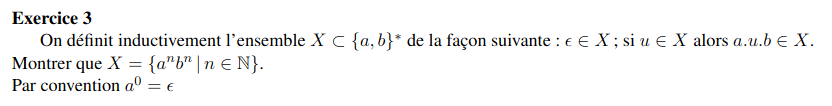
\includegraphics[scale = 0.6]{./2.png}

\noindent
\underline{Montrons que $X \subset \{a^n b^n | n \in \mathbb{N}\}$}

\

Nous allons faire une preuve par induction. Il faut donc montrer:

\begin{itemize}
    \item B'': $\epsilon \in \{a^n b^n | n \in \mathbb{N}\}$ 
    \item I'': si $u \in X$ et $u \in \{a^n b^n | n \in \mathbb{N}\}$ alors $a.u.b \in \{a^n b^n | n \in \mathbb{N}\}$
\end{itemize}

B'' est vrai puisque par convention: $a^0b^0=\epsilon \epsilon = \epsilon$.

\

I'' est vrai puisque si $u \in \{a^n b^n | n \in \mathbb{N}\}$ alors $\exists n_0 \in \mathbb{N}$ tel que $u = a^{n_0}b^{n_0}$ et donc: \\
$a.u.b = a^{n_0 + 1}b^{n_0 +1 } \in \{a^n b^n | n \in \mathbb{N}\}$. 

\

\noindent
\underline{Montrons que $\{a^n b^n | n \in \mathbb{N}\} \subset X$}

\

Nous allons faire une preuve par récurrence. Soit $n \in \mathbb{N}$, on pose comme hypothèse de récurrence:

\begin{equation*}
    H_n\text{ : } a^nb^n \in X
\end{equation*}

\underline{Initialisation}: $a^0b^0 = \epsilon \in X$.

\

\underline{Hérédité}: Soit $k \in \mathbb{N}$ tel que $(H_k)$. On a $a^kb^k \in X$ donc, par application de la règle I, on a $a^{k+1}b^{k+1} \in X$. $(H_{k+1})$ est prouvé.

\

\underline{Conclusion}: Notre récurrence démontre que $\forall n \in \mathbb{N}, a^nb^n \in X$, donc $\{a^n b^n | n \in \mathbb{N}\} \subset X$.

\

Finalement, on a donc montré que: $$X = \{a^n b^n | n \in \mathbb{N}\} $$

\

\subsection{Exercice 6 du TD1}

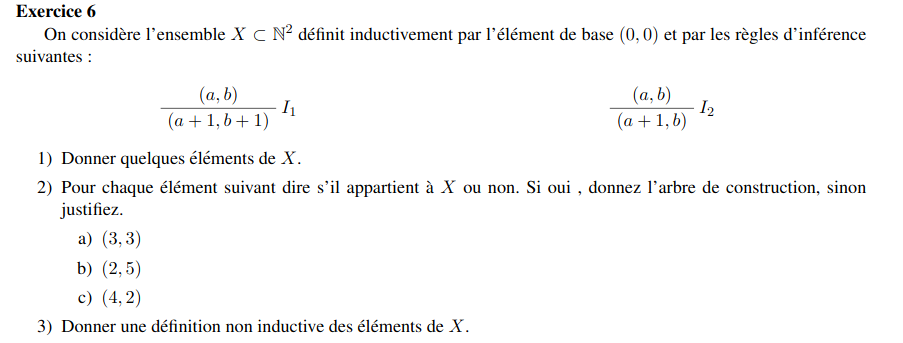
\includegraphics[scale = 0.5]{./3.png}

\

\noindent
2) Élément $(3,3)$

\begin{prooftree}
\AxiomC{$(0,0)$}
\RightLabel{$(I_1) * 3$}
\UnaryInfC{$(3,3)$}
\end{prooftree}

\noindent
2) Élément $(2,5)$

\

Pour démontrer que $(2,5)$ n'est pas dans X, on va prouver par induction, la proposition suivante (rigoureusement ce devrait être un prédicat mais on peut se permettre quelques approximations):

\begin{equation*}
    (P): \forall (x,y) \in X, x \geq y 
\end{equation*}

\

B'' : $0 \geq 0$ est immédiatement vérifié.

\

$I_1$'':  si $a \geq b$ alors $a + 1 \geq b + 1$: $I_1''$ est vérifié.

\

$I_2''$: si $a \geq b$ alors $a + 1 \geq b$: $I_2''$ est vérifié.

\

Par notre preuve par induction, si $(x,y) \in X$, alors $ x \geq y$ donc $(2,5) \not\in X$.

\

\noindent
2) Élément $(4,2)$


\begin{prooftree}
\AxiomC{$(0,0)$}
\RightLabel{$(I_2) * 2$}
\UnaryInfC{$(2,0)$}
\RightLabel{$(I_1) * 2$}
\UnaryInfC{$(4,2)$}
\end{prooftree}

\

\noindent
3)

\

Montrons que $X = \{ (x,y) \in \mathbb{N}^2 / x \leq y \}$. On a déjà montré que $X \subset \{ (x,y) \in \mathbb{N}^2 / x \geq y \}$, il ne reste donc que l'autre inclusion à démontrer.

\

\noindent
\underline{Montrons que $\{ (x,y) \in \mathbb{N}^2 / x \geq y \} \subset X$}

\

Soit $(a,b) \in \{ (x,y) \in \mathbb{N}^2 / x \geq y \}$. Quelque soit les éléments $a,b$ on peut leur donner un arbre de construction:

\begin{prooftree}
\AxiomC{$(0,0)$}
\RightLabel{$(I_1) * b$}
\UnaryInfC{$(b,b)$}
\RightLabel{$(I_2) * (a-b)$}
\UnaryInfC{$(a,b)$}
\end{prooftree}

\

Donc tous les couples $(a,b)$ tels que $a \geq b$ sont des théorèmes; ce qui montre que $\{ (x,y) \in \mathbb{N}^2 / x \geq y \} \subset X$. 

\

\subsection{Exercice 1.5 du livre (page 57)}

\noindent
\underline{Sujet}: Montrer que le nombre de sous-formules d'une formule $F$ est inférieur ou égal à $2^{\tau(F) +1} -1$.

\

Re-définissons tout d'abord \textbf{inductivement}, l'ensemble des formules que nous noterons $F_a$.

\begin{prooftree}
\AxiomC{$F$ est atomique}
\RightLabel{$(B)$}
\UnaryInfC{$F \in F_a$}
\end{prooftree}

\begin{prooftree}
\AxiomC{$F \in F_a$}
\RightLabel{$(I_1)$}
\UnaryInfC{$QF \in F_a$}
\end{prooftree}

\begin{prooftree}
\AxiomC{$F \in F_a$}
\RightLabel{$(I_2)$}
\UnaryInfC{$\neg F \in F_a$}
\end{prooftree}

\begin{prooftree}
\AxiomC{$F_1 \in F_a$}
\AxiomC{$F_2 \in F_a$}
\RightLabel{$(I_3)$}
\BinaryInfC{$F_1 \oplus F_2 \in F_a$}
\end{prooftree}

\

Faisons une preuve par induction de la proposition en jeu:

\

\textit{Notation}: $ns(F) = Card(SF(F))$

\

B'': si $F$ est atomique on sait que $\tau(F) = 1$, donc $2^{\tau(F) + 1} - 1 = 1$. On sait aussi que $SF(F) = \{F\}$ donc $ns(F) = 1$ ce qui donne bien $ns(F) \leq 2^{\tau(F) + 1} - 1$.

\

$I_1''$: \textbf{si} $ns(F) \leq 2^{\tau(F) + 1} - 1$ \textbf{alors} $ns(QF) \leq 2^{\tau(QF) + 1} - 1$. Preuve:

\

Comme on sait que $\tau(QF) = 1 + \tau(F)$, on a:

\begin{equation*}
    ns(QF) = ns(F) + 1 \leq 2^{\tau(F) + 1} \leq 2^{\tau(F) + 2} - 1 = 2^{\tau(QF) + 1} - 1
\end{equation*}

\

$I_2''$: Analogue à la preuve de $I_1''$ (on peut le voir en "remplacant" Q par $\neg$)

\

$I_3''$: Supposons que $ns(F_1) \leq 2^{\tau(F_1) + 1} - 1$ et que $ns(F_2) \leq 2^{\tau(F_2) + 1} - 1$.

\

On sait que $SF(F_1 \oplus F_2) = \{F_1 \oplus F_2\} \cup SF(F_1) \cup SF(F_2)$ donc: \begin{align*}
    ns(F_1 \oplus F_2) = 1 + ns(F_1) + ns(F_2) &\leq 1 + 2^{\tau(F_1) + 1} - 1 + 2^{\tau(F_2) + 1} - 1 \\
    &= 2^{\tau(F_1 \oplus F_2) - \tau(F_2)} + 2^{\tau(F_1 \oplus F_2) - \tau(F_1)} - 1 \\
    &\leq 2*2^{\tau(F_1 \oplus F_2) - \min(\tau(F_1),\tau(F_2))} - 1 \\
     &\leq 2^{\tau(F_1 \oplus F_2) + 1} - 1
\end{align*}

\

car $\tau(F_1 \oplus F_2) = 1 + \tau(F_1) + \tau(F_2)$ et $\min(\tau(F_1),\tau(F_2)) \geq 0$.

\section{Les Démonstrations}


\subsection{Les séquents}

On démontre, en général, des formules en utilisant un ensemble d'hypothèses, et cet ensemble peut varier en cours de la démonstration: quand on dit "supposons $F$ et montrons $G$", $F$ est alors une nouvelle hypothèse que l'on pourra utiliser pour montrer $G$. Pour formaliser cela, on introduit la notion de séquent.

\

\begin{tcolorbox}
    \textbf{Définition:} Un  \textit{séquent} est un couple (noté $\Gamma \vdash F$) où:
    
    \begin{itemize}
        \item $\Gamma$ est un ensemble \textit{fini} de formules. $\Gamma$ représente les hypothèses que l'on peut utiliser. Cet ensemble s'appelle aussi le \textit{contexte} du séquent.
        \item $F$ est une formule. C'est la formule que l'on veut montrer. On dira que cette formule est la \textit{conclusion} du séquent.
    \end{itemize}
\end{tcolorbox}

\

\begin{tcolorbox}
    \textbf{Définition:} Un séquent $\Gamma \vdash F$ est \textit{prouvable} (ou \textit{démonstrable} ou \textit{dérivable}) s'il peut être obtenu par une appliciation finie de règles décrites dans la section suivante. Une formule $F$ est \textit{prouvable} si le séquent $\vdash F$ est prouvable.
\end{tcolorbox}

\

\noindent
\textit{Remarques:}

\begin{itemize}
    \item $"\Gamma \vdash F"$ représente à la fois le séquent et la phrase $"\Gamma \vdash F$ est prouvable". Il n'y aura, en général, pas d'ambiguïté.
    \item On écrira $\Gamma \not\vdash F$ pour dire "$\Gamma \vdash F$ n'est pas prouvable".
    \item Il existe des systèmes de démonstration qui n'utilisent pas ce principe hypothèses/conclusions (par exemple le système d'Hilbert).
\end{itemize}

\subsection{Rappel: démonstration formelle d'une formule}

Rappelons comment construire un arbre de preuve pour démontrer une formule classique: \\
$\neg A \leftrightarrow (A \rightarrow \bot)$.

\

Avant de commencer, définissions une règle d'introduction de $\leftrightarrow$:

\begin{prooftree}
\AxiomC{$\vdash A \rightarrow B$}
\AxiomC{$\vdash B \rightarrow A$}
\RightLabel{$\leftrightarrow_i$}
\BinaryInfC{$\vdash A \leftrightarrow B$}
\end{prooftree}

Cette règle se déduit naturellement de l'introduction de la conjonction et du fait que: \\
$A \leftrightarrow B \equiv (A \rightarrow B) \land (B \rightarrow A)$

\

A partir de là, on peut écrire l'arbre de $\neg A \leftrightarrow (A \rightarrow \bot)$:

\begin{prooftree}
\AxiomC{$A \rightarrow \bot, A \vdash A \rightarrow \bot$}
\AxiomC{$A \rightarrow \bot, A \vdash A$}
\RightLabel{$\rightarrow_e$}
\BinaryInfC{$A \rightarrow \bot, A \vdash \bot$}
\RightLabel{$\neg_i$}
\UnaryInfC{$A \rightarrow \bot \vdash \neg A$}
\RightLabel{$\rightarrow_i$}
\UnaryInfC{$\vdash (A \rightarrow \bot) \rightarrow \neg A$}
\AxiomC{$\neg A, A \vdash \neg A$}
\AxiomC{$\neg A, A \vdash A$}
\RightLabel{$\neg_e$}
\BinaryInfC{$\neg A, A \vdash \bot$}
\RightLabel{$\rightarrow_i * 2$}
\UnaryInfC{$\vdash \neg A \rightarrow (A \rightarrow \bot)$}
\RightLabel{$\leftrightarrow_i$}
\BinaryInfC{$\vdash \neg A \leftrightarrow (A \rightarrow \bot)$}
\end{prooftree}

\

\section{Complétude de la logique du premier ordre}

\subsection{Interprétations}

Dans cette section, on définit la \textit{vérité} d'une formule, ce qui nécessite la notion d'\textbf{interprétation} d'un langage.

\

\begin{tcolorbox}
    \textbf{Définition:} Soit $L$ un langage de la logique du premier ordre. On appelle \textit{interprétation} du langage $L$, l'ensemble $M$ des données suivantes:
    
    \begin{itemize}
        \item Un ensemble non vide $|M|$, appelé \textit{domaine} ou \textit{ensemble de base} de $M$.
        \item pour chaque symbole de constante $c$, un élément $c_M$ de $|M|$.
        \item pour chaque symbole de fonction $n$-aire $f$, une fonction $f_M$, partout définie, de $|M|^n$ dans $|M|$
        \item pour chaque symbole de relation $n$-aire $R$ (autre que =) un sous ensemble $R_M$ de $|M|^n$.
    \end{itemize}
\end{tcolorbox}

\

\noindent
\textit{Remarques:}

\begin{itemize}
    \item On utilise quelquefois les mots \textit{structure} ou \textit{modèle}, avec le même sens, à la place du mot \textit{interprétation}
    \item Donner une interpétation consiste donc à dire dans quel ensemble on travaille et ce que représente les symboles utilisés. L'hypothèse $|M|$ non vide, outre le fait qu'une interprétation vide n'est pas très intéressante, est nécessaire pour avoir le \textbf{théorème de complétude}. En effet, si on veut qu'une formule démontrable soit vraie dans tout interpétation, il faut, à cause de la règle $\exists_i$, que $|M|$ soit non vide.
    \item Par convention: $|M|^0 = \emptyset$
    \item \textbf{Pour simplifier les notations, on confondra souvent une interprétation avec son ensemble de base}. C'est une pratique courante en mathématique: quand on parle de l'espace vectoriel $\mathbb{R}^n$ on ne précise pas ce qu'est l'addition et le produit par un scalaire. On dira donc souvent "soit $M$ une interprétation" sans préciser d'avantage.
\end{itemize} 

\

\begin{tcolorbox}
    \textbf{Définition:} Soit $M$ une interprétation du langage $L$.
    
    \
    
    1. Un \textit{environnement} est une fonction de l'ensemble des variables dans $|M|$, l'ensemble de base de $M$. 

    \
    
    2. Si $e$ est un environnement et $a \in |M|$, on note $e[x:=a]$ l'environnement $e'$ tel que $e'(x) = a$ et $e'(y) = y$ pour $y$ différent de $x$.

\end{tcolorbox}

\

\begin{tcolorbox}
    \textbf{Définition:} Soit $M$ une interprétation du langage $L$. La \textit{valeur} du terme $t$ dans l'environnement $e$ (on la note $\text{Val}_M(t,e)$) est définie, par récurrence sur la taille de $t$, de la manière suivante:
    
    \begin{itemize}
        \item $\text{Val}_M(c,e) = c_M$
        \item $\text{Val}_M(x,e) = e(x)$ si $x$ est une variable
        \item $\text{Val}_M(f(t_1, ..., t_n),e) = f_M(\text{Val}_M(t_1,e), ..., \text{Val}_M(t_n,e))$
    \end{itemize}

\end{tcolorbox}

\

\noindent
\underline{Exemple}: Soit $L = \{0, 1, +, *, =\}$ le langage de l'arithmétique.

\

On peut prendre comme interprétation l'ensemble $\mathbb{N}$ en interprétant les symboles dans leur sens habituel.

\

On peut également prendre $\mathbb{Z} \text{ (ou } \mathbb{R}, \mathbb{Q}, \mathbb{C}...$) en interprétant les symboles avec leur sens habituel.

\

Mais on peut aussi prendre l'interpétation $M$ définie par $|M| = \mathbb{N}$, $0_M = 1_M = 18$ et $n +_M m = 3.n + 5.m$. Ce qui donne par exemple: $0_M +_M 3 = 3*18 + 5*3 = 69$.

\

\begin{tcolorbox}
    \textbf{Lemme}: $\text{Val}_M(t,e)$ ne dépend que de la valeur de $e$ sur les variables de $t$ 
\end{tcolorbox}

\

\noindent
\textit{Notation}:  Pour simplifier les notations, on évitera de noter l'indice $M$ ou le paramètre $e$ quand le contexte est suffisamment clair. On pourra donc noter  $\text{Val}(t,e)$ ou encore $\text{Val}(t)$.

\

\begin{tcolorbox}
    \textbf{Définition:} Soit $M$ une interprétation du langage $L$. La valeur d'une formule $F$ de $L$ dans l'environnement $e$ est un élement de l'ensemble $\{0,1\}$ noté $\text{Val}_M(F,e)$ (que l'on notera ici $\text{Val}(F)$) et défini, par récurrence sur la taille de $F$, de la manière suivante:
    
    \begin{itemize}
        \item $\text{Val}(\bot) = 0$
        \item $\text{Val}(R(t_1, ..., t_n)) = 1$ ssi $(\text{Val}(t_1), ..., \text{Val}(t_n)) \in R_M$
        \item $\text{Val}(\neg F_1) = 1$ ssi $\text{Val}(F_1) = 0$
        \item $\text{Val}(F_1 \land F_2) = 1$ ssi $\text{Val}(F_1) = 1$ et $\text{Val}(F_2) = 1$ 
        \item $\text{Val}(F_1 \lor F_2) = 1$ ssi $\text{Val}(F_1) = 1$ ou $\text{Val}(F_2) = 1$ \item $\text{Val}(\forall x F_1) = 1$ ssi pour tout $a \in |M|$, $\text{Val}(F_1, e[x:=a]) = 1$
        \item $\text{Val}(\exists x F_1) = 1$ ssi il existe $a \in |M|$, $\text{Val}(F_1, e[x:=a]) = 1$
    \end{itemize}

\end{tcolorbox}

\newpage

\noindent
\textit{Remarques et notations}

\

1. Les définitions précédentes peuvent paraître triviales, mais cette trivialité apparente vient seulement du fait que les connecteurs et les quantificateurs ont pour nous leur sens "courant". On notera qu'on a, par exemple, écrit $\land$ pour designer le connecteur qui apparaît dans une formule, mais on a utilisé le mot "ou" quand on définit son sens: c'est alors, intuitivement, le "ou" de notre méta-langage.

\

2. De même que formules et termes sont des objets de nature différentes, leur valeur est aussi de valeur différente: la valeur d'un terme est un élément du domaine $|M|$ alors que la valeur d'une formule est un booléen (0 représentant le faux et 1 le vrai).

\

3. Dans le cas d'un symbole $R$ de relation d'arité $0$ (une variable propositionnelle) on conviendra que $\text{Val}_M(R) = 1$ si $R_M = \{\emptyset \}$ et $Val_M(R) = 0$ si $R_M = \emptyset$. En effet, $|M|^0 = \{\emptyset \}$ et on peut identifier ses sous ensembles à $\{0,1\}$

\

4. \colorbox{yellow}{On notera souvent $M, e \Vdash F$ (ou même $M \Vdash F$ si l'environnement est clair)} au lieu de $\text{Val}_M(F,e) = 1$. De la même façon, on notera $M, e \not\Vdash F$ (ou 
$M \not\Vdash F$) à la place de $\text{Val}_M(F,e) = 0$. Ainsi, au lieu de dire "la valeur de $F$ dans l'environnement $e$ est 1 (resp. 0)" on dira plutôt "$M$ satisfait (resp. ne satisfait pas) $F$ dans l'environnement $e$". Si $M \Vdash F$, on dit aussi que $M$ est un \textit{modèle} de F.

\

5. Il résulte immédiatement de la définition que, pour tout environnement $e$, on a: $M, e \Vdash F$ ou $M, e \not\Vdash F$. Il est également facile de voir que $M, e \Vdash \neg F$ ssi $M, e \not\Vdash F$. Donc on ne peut pas avoir simultanément $M , e \Vdash F$ et $M , e \Vdash \neg F$.

\

\begin{tcolorbox}
    \textbf{Lemme}: $\text{Val}_M(F,e)$ ne dépend que de la valeur de $e$ sur les variables \textbf{libres }de $F$.
    
    \
    
    \textbf{Corollaire}: Si $F$ est une formule close, alors la valeur de $F$ est indépendante de l'environnement. On note alors $M \Vdash F$.
\end{tcolorbox}

\

\noindent
\underline{Exemple}:

\

Soit $L = \{ e, f \}$ le langage où $e$ est un symbole de constante et $f$ est un symbole de fonction binaire. On définit les interprétations $N$ et $Z$ par :

\begin{itemize}
    \item $|N| = \mathbb{N}$, $e_N = 0$ et $f_N(a,b) = a+b$
    \item $|Z| = \mathbb{Z}$, $e_Z = 0$ et $f_Z(a,b) = a+b$
\end{itemize}

Considérons les formules:
$$ F: \forall x, y, z \{ f(x,f(y,z)) = f(f(x,y),z)$$
$$ G: \forall x \{f(e,x) = x \land f(x,e) = x\} $$
$$ H: \forall x \exists y \{f(x,y) = e \land f(y,x) = e\} $$

\

On sait que $M \Vdash F$ ssi pour tout élément $a, b, c$ de $|M|$ on a $f_M(a,f_M(b,c)) = f_M(f_M(a,b),c)$. $F$ exprime donc le fait que $f_M$ est une opération associative dans $|M|$. $G$ exprime le fait que $e_M$ est un élement neutre pour $f_M$ dans $|M|$ et H exprime le fait que tout élement de $|M|$ a un inverse pour $f_M$.

\

Donc: $N \Vdash F$, $N \Vdash G$, $N \not\Vdash H$ et $Z \Vdash F$, $Z \Vdash G$, $Z \Vdash H$

\

\

\begin{mybox}{red}{\textbf{Définition d'un théorème}}

    On dit qu'une formule $F$ est un \textit{théorème} ssi pour toute interprétation $M$ et tout environnement $e$, $M$ satisfait $F$ dans l'environnement $e$ ($M, e \Vdash F)$.

\end{mybox}

\

En d'autres mots, les théorèmes sont les formules \textit{toujours} vraies, c'est à dire quelque soit le sens qu'on donne aux objets, fonctions et relations ($\approx$ quelque soit l'interprétation, aussi appelé \textbf{modèle} dans ce contexte, sachant qu'on néglige un peu l'environnement). 

\

\noindent
\underline{Exemple}:

\

Soit $L = \{e, *\}$ où $e$ est une constante et $*$ un symbole de fonction binaire. Soit $A$ la formule suivante:

$$
    \forall x,y,z \{ (x*y)*z = x*(y*z) \land e*x = x \land x*e=x \land \exists x' (x' * x = e \land x * x' = e) \}
$$

\

\underline{Il est clair que chaque modèle de A est un groupe}. Maintenant, soit la formule $B$:

$$
    \forall e' \{\forall x [e' * x = x \land x * e' = x] \rightarrow e = e' \}
$$

B est la formule qui exprime l'unicité de l'élement neutre. \textbf{On a donc la formule $A \rightarrow B$ qui est un théorème.} 

\

\begin{tcolorbox}
    \textbf{Définition}: Soient $L$ et $L'$ deux langages.
    
    \begin{itemize}
        \item On dit que $L'$ \textit{enrichit} $L$ (ou que $L$ est une \textit{réstriction} de $L'$) si $L \subset L'$.
        \item On suppose $L \subset L'$. Soient $M$ une interprétation de $L$ et $M'$ une interprétation de $L'$. On dit que $M'$ est un \textit{enrichissement} de $M$ (ou que $M$ est une restriction de $M'$) ssi $|M| = |M'|$ et chaque symbole de constante, de fonction ou de relation de $L$ a la même interprétation dans $M$ et dans $M'$. 
    \end{itemize}
\end{tcolorbox}

\

\begin{tcolorbox}
    \textbf{Propriété}: Soient $L \subset L'$ deux langages et $M$ (resp. $M'$) une interprétation de $L$ (resp. $L'$). Si $M'$ est un enrichissement de $M$ et $e$ un environnement, alors:
    
    \begin{itemize}
        \item Si $t$ est un terme de $L$, $\text{Val}_M(t,e) = \text{Val}_{M'}(t,e)$.
        \item Si $F$ est une formule de $L$, alors $M,e \Vdash F$ ssi $M',e \Vdash F$.
    \end{itemize}
\end{tcolorbox}

Ainsi, la vérité d'une formule dans une interpétation ne dépend que de la restriction de cette interpétation au langage de la formule. \textbf{On peut donc parler d'une interpétation $M$ d'une formule sans dire de quel langage elle est une interpétation.}

\subsection{Introduction à la théorie des modèles}

Dans un cours de mathématiques, on étudie les propriétés de certaines structures: groupes, annaux, corps, espaces vectoriels, ect.

\

Certaines notions sont omniprésentes, par exemple celles de morphisme et d'isomorphisme. Pour d'autres, le mot utilisé dépend du type de la structure: sous-groupe, sous-espace vectoriel ect.

\

La théorie des modèles est l'étude générale des structures mathématiques. Dans cette séction on étudie quelques-unes de ces propritétés. La proposition qui suit la première définition, sera utile pour simplifier certaines preuves:

\

\begin{tcolorbox}
    \textbf{Définition}: Deux formules $F$ et $G$ sont \textit{équivalentes} ssi la formule $F \leftrightarrow G$ est un théorème; ie. ssi pour toute interpétation $M$ et tout environnement $e$: $M, e \Vdash F$, soit $\text{Val}_M(F, e) = 1$.
\end{tcolorbox}

\begin{tcolorbox}
    \textbf{Proposition}: Toute formule est équivalente à une formule n'utilisant que les connecteurs $\neg$, $\lor$ et le quantificateur $\exists$.
\end{tcolorbox}

\noindent
\underline{Preuve}: Cela résulte des équivalences suivantes pour les formules quelconques $A$ et $B$:
\begin{itemize}
    \item $A \land B$ avec $\neg(\neg A \lor \neg B)$.
    \item $A \rightarrow B$ avec $\neg A \lor B$.
    \item $\forall x A$ avec $\neg \exists x \neg A$.
\end{itemize}

Pour finir la preuve il faut donc prouver ces équivalences suivant la définition précédente de l'équivalence (cf. livre page 76)

\

\begin{mybox}{red}{\textbf{Définition d'un morphisme et d'un isomorphisme}}
    Soient $M$ et $N$ deux interpétations d'un langage $L$.
    
    \begin{itemize}
        \item Un $L$-morphisme de $M$ dans $N$ est une fonction $\phi: |M| \rightarrow |N|$ tele que:
        \begin{itemize}
            \item Pour chaque symbole de constante $c$ on a: $\phi(c_M) = c_N$
            \item Pour chaque symbole de fonction $n$-aire $f$ et pour $a_1, ... a_n \in |M|$ on a: $\phi(f_M(a_1,...,a_n)) = f_N(\phi(a_1), ..., \phi(a_n))$.
            \item Pour chaque symbole de relation $n$-aire de $R$ (autre que $=$) et pour $a_1, ... a_n \in |M|$ on a: $(a_1, ..., a_n) \in R_M$ ssi $(\phi(a_1), ..., \phi(a_n)) \in R_N$. 
        \end{itemize}
        \item Un $L$-isomorphisme est un $L$-morphisme bijectif.
        \item $M$ et $N$ sont $L$-isomorphes s'il existe un $L$-isomorphisme de $M$ dans $N$.
    \end{itemize}
\end{mybox}

\noindent
\underline{Remarque et exemple}

\begin{itemize}
    \item La notion de morphisme dépend du langage. Soit $L = \{0, +, -, \times\}$ et $L' = \{1\} \cup L$. Soient $\mathbb{Z}/3\mathbb{Z}$ et $\mathbb{Z}/12\mathbb{Z}$ les interprétations usuelles. La fonction $\phi: n \rightarrow 4n$ de $\mathbb{Z}/3\mathbb{Z}$ dans $\mathbb{Z}/12\mathbb{Z}$ est un $L$-morphisme puisque $\phi(0_L) = 0_L' = 0_L$, $\phi(0_M +_M 0_M) = \phi(0_M) +_N \phi(0_M) = 0_M +_M + 0_M = 0_M = 4*0_M$ ect. Par contre, $\phi$ n'est pas $L'$-morphisme puisque $\phi(1_M) = 4 \neq 1_N$.
\end{itemize}

En guise d'exemple, on peut vérifier que si $L = \{c,f,S\}$ et $M$ et $N$ sont définies par:

\begin{itemize}
    \item $|M| = \mathbb{R}, c_M = 0, f_M(a,b) = a + b$ et $S_M = \{(a,b) / a \leq b\}$
    \item $|N| = ]0, \infty [, c_N = 1, f_N(a,b) = ab$ et $S_N = \{(a,b) / a \leq b \}$
\end{itemize}

Alors la fonction $\phi : x \rightarrow e^{x}$ est un isomorphisme de $M$ dans $N$.

En effet:

\begin{itemize}
    \item $\phi(c_M) = c_N$ est vérifié puisque $e^0 = 1$.
    \item $\phi(f_M(a,b)) = f_N(\phi(a),\phi(b))$ est vérifié puisque $e^{a + b} = e^ae^b$
    \item $a,b \in S_M \text{ ssi } \phi(a),\phi(b) \in S_N$ est aussi vérifié puisque $a \leq b$ ssi $e^a \leq e^b$ par croissance de la fonction exponentielle.
\end{itemize}

\begin{tcolorbox}
    \textbf{Proposition}: 
    
    \begin{itemize}
        \item La composée de deux morphismes est un morphisme.
        \item La composée de deux isomorphismes est un isomorphisme.
        \item L'inverse d'un isomorphisme est un isomorphisme.
    \end{itemize}
    
\end{tcolorbox}

\

\noindent
\underline{Notation:} Si $\phi$ est un isomorphisme de $M$ dans $N$ et $e$ un environement dans $M$, on notera $\phi(e)$ l'environnement $e'$ dans $N$ défini par: $e'(x) = \phi(e(x))$ pour toute variable $x$. 

\

\begin{tcolorbox}
    \textbf{Lemme}: Soient $M$ et $N$ des interprétations d'un langage $L$ et $\phi$ un morphisme de $M$ dans $N$. Pour tout terme $t$ et tout environnement $e$ dans $M$ on a:
\begin{center} 
    $\phi(\text{Val}_M(t,e)) = \text{Val}_N(t, \phi(e))$.
\end{center}

\end{tcolorbox}

\noindent
\underline{Preuve:}

\begin{itemize}
    \item Si $t$ est une constante, cela résulte de la définition d'un morphisme.
    \item Si $t$ est une variable $x$: $\phi(\text{Val}_M(t,e)) = \phi(e(x)) = \phi(e)(x) = \text{Val}_N(t, \phi(e))$.
    \item Si $t = f(t_1, ..., t_n)$, On a: $\text{Val}_M(t,e) = f_M(\text{Val}_M(t_1,e), ..., \text{Val}_M(t_n,e))$; on veut donc montrer que: 
    $\phi(f_M(\text{Val}_M(t_1,e), ..., \text{Val}_M(t_n,e))) = f_N(\text{Val}_N(t_1, \phi(e)),     ..., \text{Val}_N(t_n, \phi(e))) 
    $
    Ce qui par définition du morphisme, revient à:
    $
    f_M(\phi(\text{Val}_M(t_1,e)), ..., \phi(\text{Val}_M(t_n,e))) = f_N(\text{Val}_N(t_1, \phi(e)), ..., \text{Val}_N(t_n, \phi(e))) 
    $
    En appliquant les résultats précédents à $\phi(\text{Val}_M(t_i,e))$, pour chaque $i \in [1,n]$ on obtient bien la formule précédente.
\end{itemize}

\begin{tcolorbox}
    \textbf{Lemme}: Soient $M$ et $N$ des interprétations d'un langage $L$ et $\phi$ un morphisme \textbf{injectif} de $M$ dans $N$. Soit $e$ un environnement dans $M$ et $F$ une formule atomique. Alors $M, e \Vdash F$ ssi $N, \phi(e) \Vdash F$.
    
\end{tcolorbox}

\noindent
\underline{Preuve:}
On rappel qu'une formule atomique est une formule de la forme $R(t_1, ..., t_n)$ ou $R$ est un symbole de relation $n$-aire de $L$ et $t_1, ..., t_n$ sont des termes de $L$.

\

On peut donc dire que $F$ est de la forme $F = R(t_1, ..., t_n)$, avec $R$ différent de $=$.

\

Etant donné que $\phi$ est un morphisme on sait que pour $t_1, ..., t_n \in |M|$, $(t_1, ..., t_n) \in R_M$ ssi $(\phi(t_1), ..., \phi(t_n)) \in R_N$.

\

Or, $M, e \Vdash F$ ssi $(\text{Val}_M(t_1,e), ..., \text{Val}_M(t_n,e)) \in R_M$, ssi $(\text{Val}_N(t_1,\phi(e)), ..., \text{Val}_N(t_n,\phi(e))) \in R_N$ ssi $N, \phi(e) \Vdash F$ par application de la définition des morphismes (sur les rélations) rappelée ci-dessus et du lemme précédent (qui donne $(\phi(\text{Val}_M(t_1,e)), ..., \phi(\text{Val}_M(t_n,e))) \in R_M$ ssi $(\text{Val}_N(t_1, \phi(e)), ..., \text{Val}_N(t_n, \phi(e))) \in R_N$).

\

Il reste encore deux cas particuliers à traiter: pour $F = \bot$, le résultat est évident. Enfin, dans le cas où $F$ est une équation $t_1 = t_2$, on applique le lemme précédent pour dire que $\phi(\text{Val}_M(t_1,e)) = \phi(\text{Val}_M(t_2,e))$ ssi $\text{Val}_N(t_1, \phi(e)) = \text{Val}_N(t_2, \phi(e))$; c'est à dire: $\phi(e(t_1)) = \phi(e(t_2))$ ssi $\phi(e(t_1)) = \phi(e(t_2))$. JSP

\

\begin{mybox}{red}{\textbf{Théorème 1.}}
	Soient $M$ et $N$ des interpétations d'un langage $L, \phi$ un isomorphisme de $M$ dans $N$ et $F$ une formule. Soit $e$ un environnement dans $M$. Alors $M, e \Vdash \text{ ssi } N, \phi(e) \Vdash F$.

\

\noindent
\textbf{Corollaire:}

Deux interpétations isomorphes satisfont les mêmes formules closes.
\end{mybox} 

Ce corollaire est souvent utilisé pour montrer que deux interpétations (de même cardinal) ne sont pas isomorphes. C'est ainsi, par exemple qu'on montre que les groupes $\mathbb{Z}/4\mathbb{Z}$ et $\mathbb{Z}/2\mathbb{Z} \times \mathbb{Z}/2\mathbb{Z}$ ne sont pas isomorphes. En effet, le premier satisfait la formules $\exists x\{x * x \neq e\}$ contrairement au second.

Le corollaire donne une condition nécessaire pour que deux interpétations soient isomorphes. Mais il faut noter que cette condition n'est pas suffisante.

\

\begin{tcolorbox}
	\textbf{Définition:} Soient $L$ un langage, $M$ et $N$ deux interpétations de $L$. On dit que $M$ est une \textit{extension} de $N$ (ou $N$ est une \textit{sous-interpétation} de M) ssi les conditions suivantes sont satisfaites:
	\begin{itemize} 
		\item $|N| \in |M|$
		\item Pour tout symbole de constante $c$ de $L$ on a: $c_N = c_M$.
		\item Pour tout symbole de fonction $n$-aire $f$ de $L$ on a: $f_N = f_M \text{ $|$ } |N|^n.$ (fonction $f_M$ dont l'ensemble de départ est $|N|^n$ ?) On remarquera que, puisque $f_N$ est une fonction de $|N|^n$ dans $|N|$, cela implique que $f_M(|N|^n)$ est inclus dans $|N|$.
		\item Pour tout symbole de relation $n$-aire $R$ de $L$ on a: $R_N = R_M \cap |N|^n$.
	\end{itemize}
\end{tcolorbox}

\begin{tcolorbox}
\textbf{Propriété:} Soient $M$ et $N$ deux interprétations d'un langage $L$. $M$ est isomorphe à une sous-interpétation $M'$ de $N$ ssi il existe un morphisme injectif de $M$ dans $N$.
\end{tcolorbox}

\

\noindent
\underline{Remarque:} Ce résultat est beaucoup utilisé. Par exemple quand on construit axiomatiquement l'ensemble $\mathbb{Z}$ à partir de $\mathbb{N}$: on définit $\mathbb{Z}$ comme le quotient de $\mathbb{N} \times \mathbb{N}$ par une relation d'équivalence. On définit ensuite une fonction de $\mathbb{N}$ dans $\mathbb{Z}$ et on vérifie que c'est un morphisme injectif. On convient alors de dire que $\mathbb{N}$ est un sous-ensemble de $\mathbb{Z}$.

\subsection{Théorème de complétude}

\

\begin{tcolorbox} 
	\textbf{Définition:} Une \textit{théorie} est un ensemble (fini ou infini) de formules closes. Les éléments d'une théorie sont souvent appelés les \textit{axiomes} de cette théorie.	
\end{tcolorbox}

\begin{tcolorbox} 
	\textbf{Définition:} Soit $T$ une théorie.
	\begin{itemize} 
		\item Une interpétation $M$ \textit{satisfait} $T$ (on dit aussi que $M$ est un \textit{modèle} de $T$ et on note $M \Vdash T$) si $M$ satisfait toutes les formules de $T$.
		\item $T$ est \textit{contradictoire} ssi il n'existe pas de modèle de $T$.
		\item Une formule close $A$ est \textit{valide} dans $T$ (on le note $T \Vdash A$) ssi $M \Vdash A$ pour tout modèle $M$ de $T$.
	\end{itemize}
\end{tcolorbox}

\begin{tcolorbox} 
	\textbf{Définition:} Soit $T$ une théorie.

	\begin{itemize} 
		\item Soit $A$ une formule. On note $T \vdash A$ s'il existe un sous-ensemble \textit{fini} $T'$ de $T$ tel que $T' \vdash A$.
		\item On dit que $T$ est \textit{consistante} ssi $T \not\vdash \bot$.
		\item On dit que $T$ est \textit{complète} ssi $T$ est consistante et pour toute formule close $F$:\\ 
		$T \vdash F$ ou $T \vdash \neg F$
	\end{itemize}
\end{tcolorbox}

\begin{tcolorbox} 
\textbf{Propriété:} Soit $T$ une théorie complète.
	\begin{itemize} 
		\item Soient A et B des formules closes. $T \vdash A \lor B$ ssi $T \vdash A$ ou $T \vdash B$.
		\item Soit A une formule close. $T \vdash \neg A$ ssi $T \not\vdash A$.
	\end{itemize}
\end{tcolorbox}

\

\begin{mybox}{red}{\textbf{Théorème de complétude}}
	Soient $T$ une théorie et $F$ une formule close.

	\begin{equation*} 
		T \vdash F \text{ ssi } T \Vdash F.
	\end{equation*}
\end{mybox}

\

\noindent
\underline{Remarques:} \\

Il faut noter que la pluspart des théories utilisées en mathématique ne sont pas complètes. Par exemple, on peut montrer que ni la théorie $G_1$ des groupes ni celle $G_2$ des groupes commutatifs, ni celle des anneaux $A$ n'est complète.

\

Soit $U$ la formule: $\forall x,y,\{xy = yx\}.$ On a $G_1 \not\vdash U$ et $G_1 \not\vdash \neg U$ puisqu'on sait bien qu'on peut aussi bien avoir des groupes commutatifs comme des groupes qui ne le sont pas dans $G_1$. Le théorème de complétude nous donne donc $G_1 \not\Vdash U$, donc $G_1$ n'est pas complet.

\

\underline{Sur le théorème de complétude:} Ce théorème montre l'équivalence entre la notion de prouvabilité (le côté syntaxique) et la notion de vérité (le côté sémantique). $T \vdash F$ corréspond à la prouvabilité (Le séquent $T \vdash F$ est \textit{prouvable} s'il peut être obtenu par une application finie de régles issues des axiomes.) La notion de vérité équivalente à cette prouvabilité, signifie que la théorie $T$ satisfait $F$ quelque soit le sens qu'on donne aux objets, fonctions et relations.

\

\begin{mybox}{red}{\textbf{Théorème sur la consistance}}
	Une théorie $T$ est consistante ssi elle est non contradictoire.
\end{mybox}

\

\begin{tcolorbox} 
	\textbf{Corollaire:} Soit $T$ une théorie non contradictoire. Si tous les modèles de $T$ sont isomorphes, alors $T$ est complète.
\end{tcolorbox}

\

\begin{mybox}{red}{\textbf{Théorème de compacité}}
	Soit $T$ une théorie. $T$ est contradictoire ssi il existe un sous-ensemble fini de $T$ qui est contradictoire. Autrement dit: $T$ est satisfiable ssi tout sous-ensemble fini de $T$ est satisfiable.
	
\end{mybox}

\subsection{Formes Canoniques}

On montre ici que toute formule peut être mise, à équivalence près, sous certaines formes canoniques.

\begin{tcolorbox} 
	\textbf{Proposition:} Soient $A$ et $B$ des formules. Si $x$ n'est pas libre dans $B$, les formules $\forall x A \lor B \leftrightarrow \forall x (A \lor B)$ et $\exists x A \lor B \leftrightarrow \exists x (A \lor B)$ sont des théorèmes.
\end{tcolorbox}

\begin{tcolorbox} 
\textbf{Corollaire:} Soient $A$ et $B$ des formules telles que les variables $x_1, ..., x_n$ (resp. $y_1, ..., y_m$ ne sont pas libres dans $B$ (resp. $A$). Pour tout choix de quantificateurs $Q_1, ..., Q_n; P_1, ..., P_m$, la formule ci-dessous est un théorème:

\begin{center} 
		
	$Q_1 x_1 ... Q_n x_n A \lor P_1 y_1 ... P_m y_m B \leftrightarrow Q_1 x_1 ... Q_n x_n P_1 y_1 ... P_m y_m (A \lor B)$
\end{center}

\end{tcolorbox}

\subsubsection{Formules conjonctives et disjonctives}

\begin{tcolorbox} 
	\textbf{Définition:}

	\begin{itemize} 
		\item On dit que $F$ est sous formes \textit{conjonctive} si $F$ est une conjonction de disjonctions de formules atomiques ou de négations de formules atomiques. On écrira une formule conjonctive sous la forme $\land_{i}^{} \lor_{j}^{} F_{i,j}$: cela signifie donc que les formules $F_{i,j}$ sont des formules atomiques ou des négations de formules atimiques.
		\item On dit que F est sous formes \textit{disjonctive} si $F$ est une disjonction de conjonctions de formules atomiques ou de négations de formules atomiques. De même on écrira une formule disjonctive sous la forme: $\lor_{i}^{} \land_{j}{}^{} F_{i,j}$.
	\end{itemize}
\end{tcolorbox}

Exemple: $(A \land \neg B) \lor C \lor (D \land \neg A)$ est sous forme disjonctive. $(D \lor A \lor C) \land (D \lor \neg B)$ est sous formes conjonctive.

\

\begin{mybox}{red}{\textbf{Théorème}}
	Toute formule sans quantificateurs est équivalente à une formule sous forme conjonctive et à une formule sous forme disjonctive.
\end{mybox}

\subsubsection{Formules prénexes}

\begin{tcolorbox} 
	\textbf{Définition:}Une formule $F$ est sous forme \textit{prénexe} si elle est de la forme $Q_1 x_1 ... Q_n x_n G$ où $Q_i = \forall$ ou $\exists$ et G est sans quantificateurs. On dira alors que $Q_1 x_1 ... Q_n x_n$ est le préfixe de F. Le préfixe peut être vide, ie. une formule sans quantificateur est sous forme prénexe.
\end{tcolorbox}

\begin{mybox}{red}{\textbf{Théorème}}
	Toute formule est équivalente à une formule sous forme prénexe.
\end{mybox}

\

\begin{tcolorbox} 
	\textbf{Définition:} On dit qu'une formule $F$ est sous forme \textit{prénexe conjonctive} (resp. \textit{pénexe disjonctive}) ssi $F = Q_1 x_1 ... Q_n x_n G$ ou $G$ est une fomule sans quantificateur et sous forme conjonctive (resp. disjonctive)
\end{tcolorbox}

\begin{tcolorbox} 
	\textbf{Proposition:} Toute formule est équivalente à une formule sous forme prénexe conjonctive et à une formule sous forme prénexe disjonctive.
\end{tcolorbox}

\

\begin{tcolorbox} 
	\textbf{Définition:} Une formule est \textit{universelle} (resp. \textit{existentielle}) si elle est prénexe et son préfixe ne contient que des $\forall$ (resp. $\exists$)
\end{tcolorbox}


\

\begin{tcolorbox} 
	\textbf{Proposition:} Soit $N$ une sous-interpétation de $M$ et $e$ un environnement de $N$.

	\begin{itemize} 
		\item Si $t$ est un terme, alors $Val_N (t,e) = Val_M (t,e)$.
		\item Si $F$ est une formule sans quantificateur, alors $M, e \Vdash F$ ssi $ N,e \Vdash F$.
		\item Si $F$ est universelle et $M, e \Vdash F$ alors $N, e \Vdash F$.
		\item Si $F$ est existentielle et $N, e \Vdash F$ alors $M, e \Vdash F$.
	\end{itemize}
\end{tcolorbox}

\subsection{Skolémisation}

On donne, dans cette section, les résultats mathématiques qui sont à la base de plusieurs algorithmes de démonstration automatique.

\begin{tcolorbox} 
	\textbf{Définition:} Soit $F = Q_1 x_1 ... Q_n x_n G$ une formule prénexe ($Q_i = \forall$ ou $\exists$ et $G$ est sans quantificateur). Soient $i_1 < ... < i_m$ les indices tels que $Q_i = \exists$.

	\begin{itemize} 
		\item On associe à $L$ le langage $L_S(F) = L \cap \{f_1, ..., f_m\}$ où $f_1, .., f_m$ sont des nouveaux symboles de fonction (appelés \textit{fonctions de Skolem associées à F}). L'arité de $f_r$ est $i_r - r$ c'est à dire le nombre de $\forall$ situés à gauche de $Q_{i_r}$ dans le préfixe de $F$. 	
		\item Pour $1 \leq r \leq m$, on désigne par $t_r$ le terme de $L_S(F)$ obtenu en appliqant $f_r$ aux $i_r - r$ variables quantifiées universellement à gauche de $Q_{i_r}$ dans le préfixe de $F$.
		\item Une formule $F_S$ (appelée \textit{forme de Skolem} de F) est obtenue à partir de $F$ en enlevant les $\exists$ du préfixe de F et en remplaçant dans la formule $G$ chaque occurence de la variable $x_{i_r}$ par le terme $t_r$.
	\end{itemize}
\end{tcolorbox}

\noindent
\underline{Exemple:} Soit $L =\{f, R\}$ où $f$ est un symbole de fonction unaire et $R$ est un symbole de relation binaire. Soit $F: \exists x_1 \forall y_1 \forall y_2 \exists x_2\{R(x_1, f(y_1)) \land R(f(y_2),x_1) \rightarrow R(x_1, x_2)\}$

\

Ici on a $i_1 = 1$ et $i_2 = 4$. $L_S(F) = L \cap\{e, g\}$. Ici, $e$ et $g$ (les fonctions de Skolem associées à $F$) ont pour arité réspective $1 - 1 = 0$ et $4 - 2 = 2$. $e$ est donc un terme constant (fonction d'arrité 0). $g$ est le symbole de fonction qui s'appliquera à $y_1$ et $y_2$ dans la forme de Skolem de F. Ainsi, la formule $F_S$ est donc:

\begin{center} 
	$ F_S: \forall y_1 \forall y_2 \{R(e, f(y_1)) \land R(f(y_2),e) \rightarrow R(e, g(y_1, y_2))\}$
\end{center}

\begin{tcolorbox} 
	\textbf{Lemme:} Soit $F$ une formule prénexe de $L$. Alors la formule $F_S \rightarrow F$ du langage $L_S(F)$ est un théorème et, par conséquent, $\vdash F_S \rightarrow F$.
\end{tcolorbox}

\begin{tcolorbox} 
	\textbf{Lemme:} Soient $L$ un langage, $F$ une formule prénexe et $M$ une interprétation de L tels que $M \Vdash F$. Il existe un enrichissement de $M$ en une interprétation $N$ de $L_S(F)$ tel que $N \Vdash F_S$.
\end{tcolorbox}

\begin{tcolorbox} 
	\textbf{Corollaire:} Soit F une formule close prénexe et $F_S$ la forme de Skolem de $F$. $F$ admet un modèle ssi $F_S$ admet un modèle.
\end{tcolorbox}

\

C'est le théorème ci-dessous qui est la base théorique de la pluspart des algorithmes de démonstration automatique:

\begin{mybox}{red}{\textbf{Théorème}}
	Une formule close prénexe $F$ est démontrable ssi la forme de Skolem de $\neg F$ est contradictoire.
\end{mybox}

\noindent
\underline{Exemple:} Soit $F: \exists x \forall y\{R(x) \rightarrow R(y)\}$. On a donc $\neg F:\forall x \exists y\{R(x) \land \neg R(y)\}$. On a $i_1 = 2$; donc on remplace $y$ par $f(x)$ pour avoir la forme de Skolem de $\neg F$:

\begin{center} 
	$ \neg F_S: \forall x\{R(x) \land \neg R(f(x))\}$
\end{center}

Soit $M$ une interprétation et $a \in |M|$. Si $M \Vdash \neg F_S$ alors $M \Vdash R(f(a))$ et $M \Vdash \neg R(f(a))$ (pas sûr). On a donc une contradiction: F est démontrable, d'après le théorème précédent.


\section{Quelques applications sur la théorie des modèles}

\subsection{Exercice 1}

\underline{Enoncé:} Soit $L =\{0, S, +, \times\}$ où $0$ est une constante et $S$ (resp. $+$, $\times$) est un symbole de fonction unaire (resp. binaire). Soit $\mathbb{N}$ l'interpétation standard de $L$.

\

Donner la formule, écrite sur $L$ qui exprime: \textbf{p est strictement plus petit que q}.

$$F_1: \exists x, x \neq 0 \land p + x = q$$

Donner la formule, écrite sur $L$ qui exprime: \textbf{p divise q}

$$ F_2: \exists k, k \neq 0 \land p \times k = q$$

Donner la formule, écrite sur $L$ qui exprime: \textbf{p est premier}

$$ F_3: \neg (\exists a \exists b, a \times b = p \land \neg(a = p \lor b = p))$$

Donc:

$$F_3: \forall a \forall b, a \times b \neq p \lor a = p \lor b = p$$

\subsection{Exercice 2}

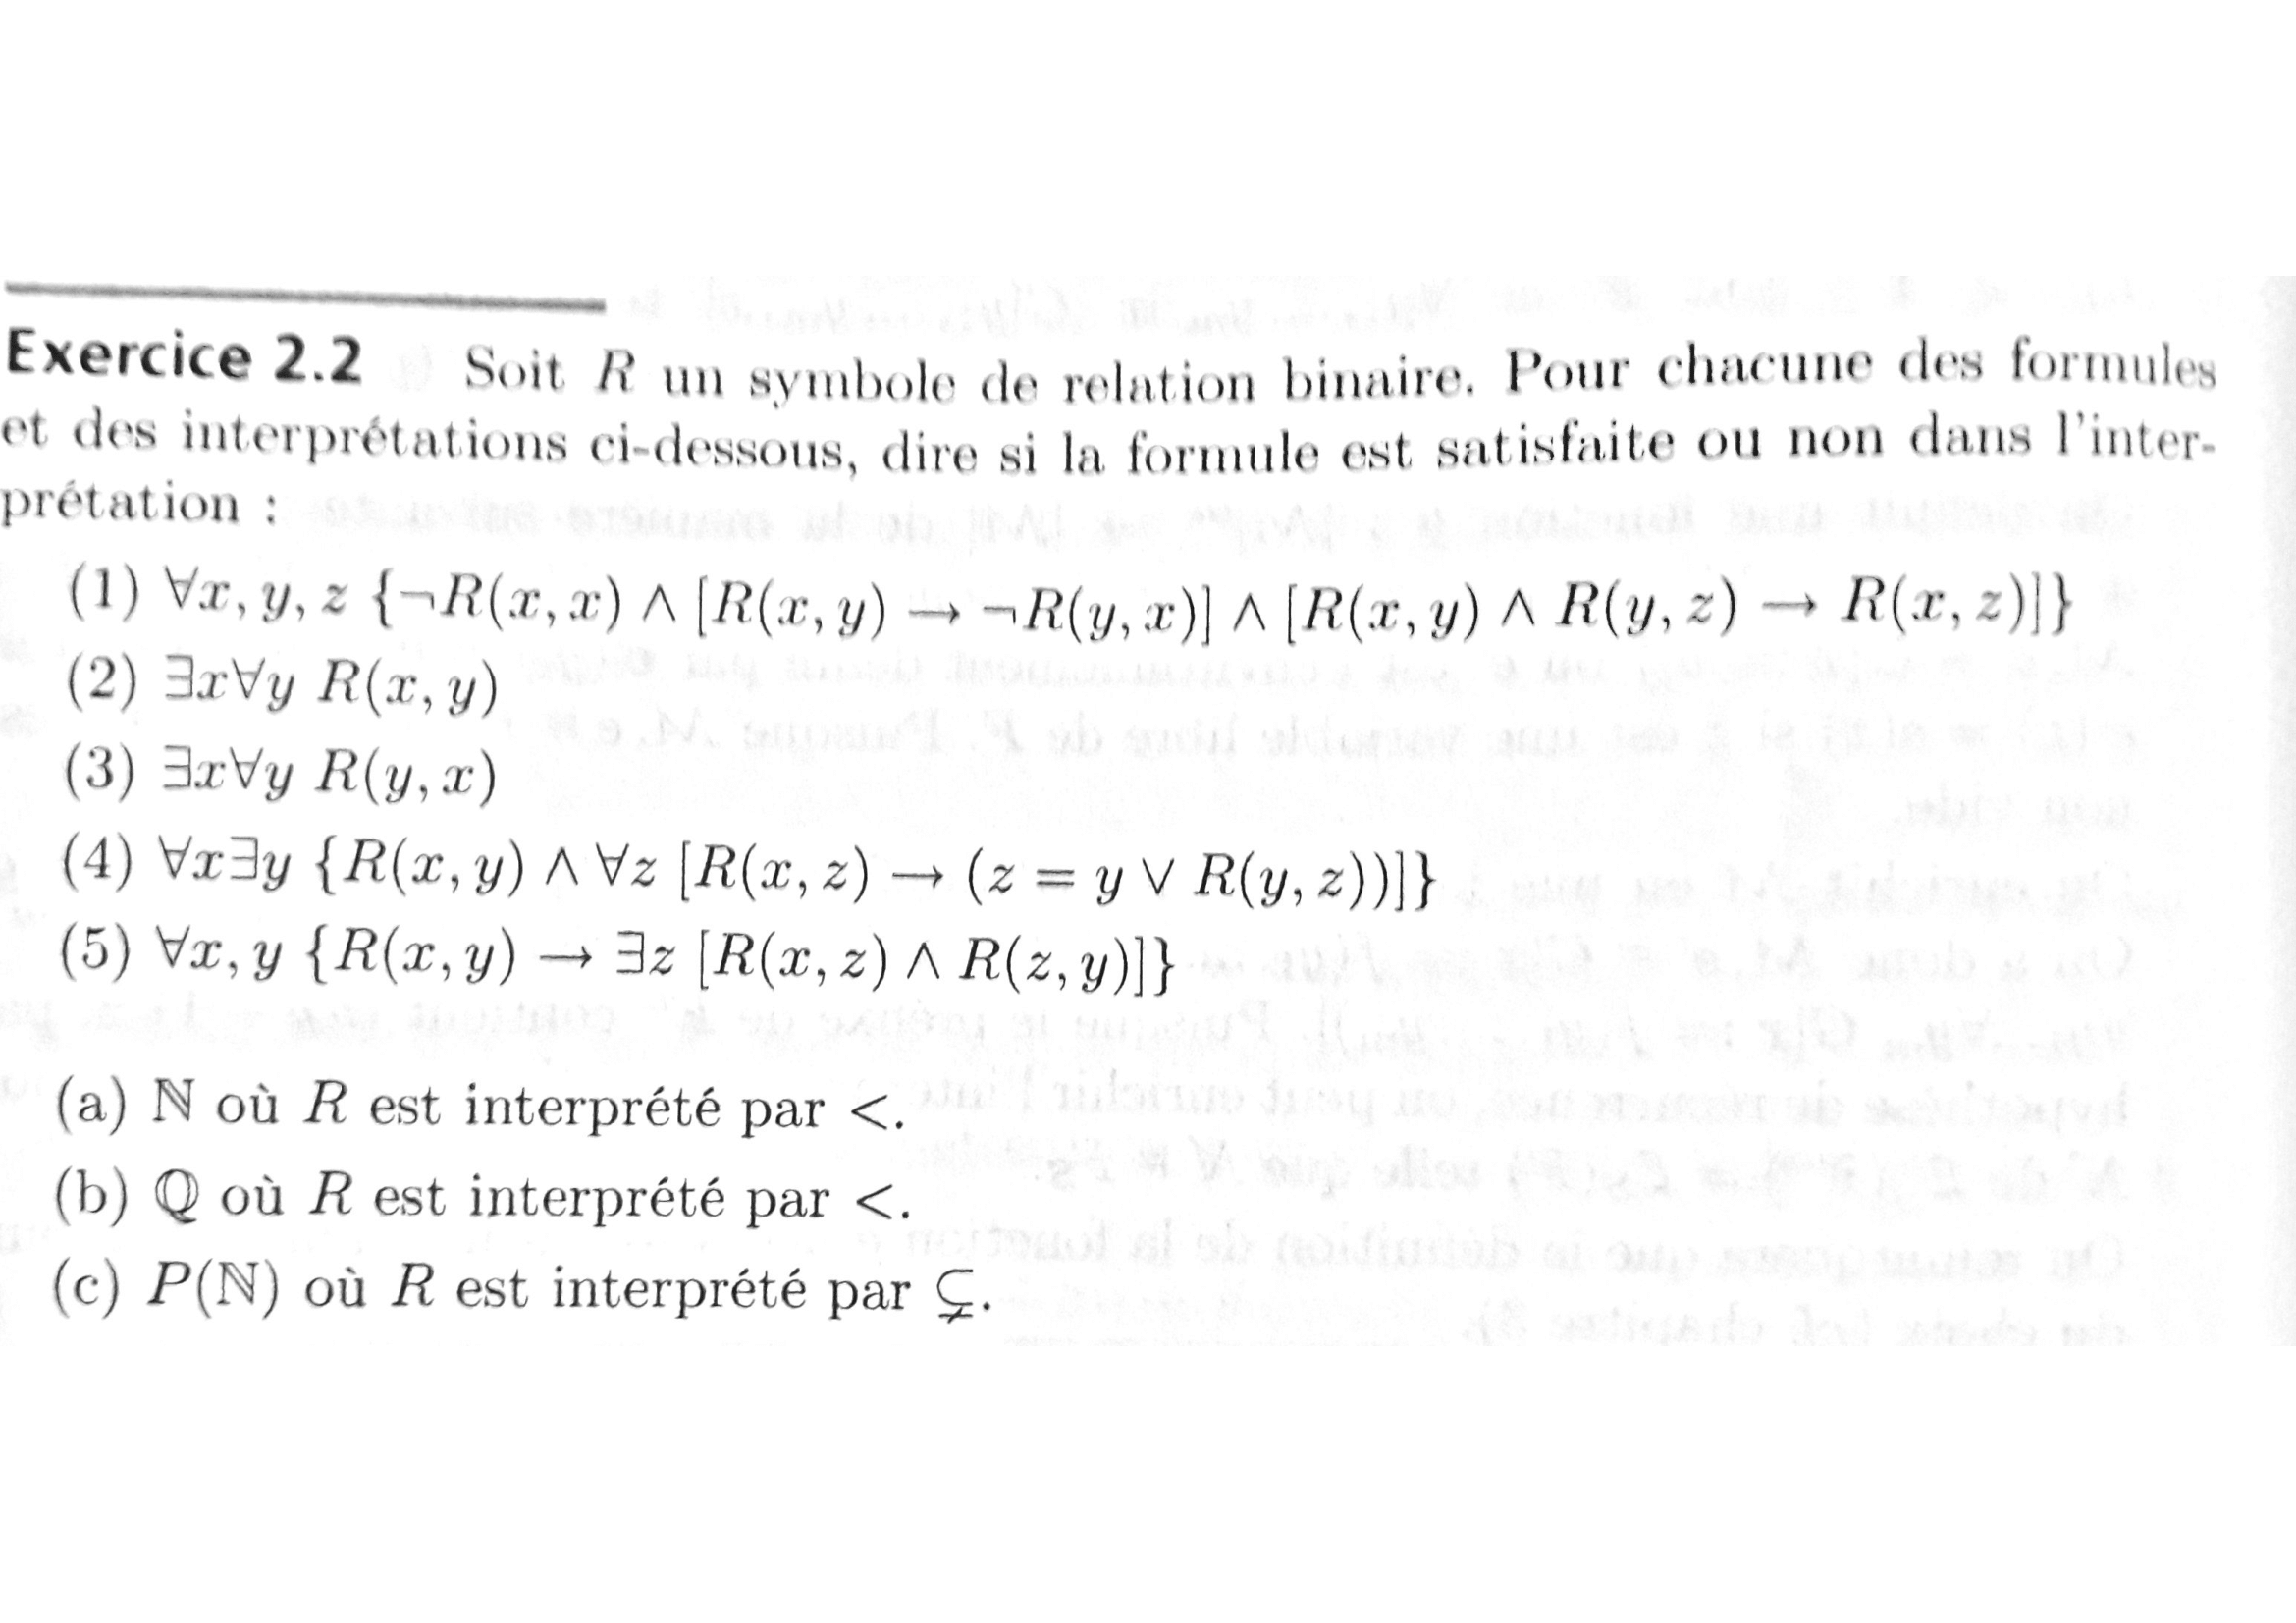
\includegraphics[scale = 0.2]{4.png}

\subsubsection{Cas (1), modèle (a)}

Avec le modèle $|M| = \mathbb{N}$, où $R$ est interpété par $<$ on a:

$\forall x,y,z\{\neg(x < x) \land (x < y \rightarrow y < x) \land (x < y \land y < z \rightarrow x < z)\}$

\

Simplifiable en:

$$\forall x,y,z\{(x < y \rightarrow y < x) \land (x < y \land y < z \rightarrow x < z)\}$$

Comme il est évident que la première condition dans le $\land$ est fausse; cette formule n'est pas satisfiable selon ce modèle.

\subsection{Exercice 3}

Le but de cet exercice est de montrer qu'en logique du premier ordre on peut se passer des symboles de fonctions: il suffit, intuitivement, de remplacer une fonction par son graphe.

\

Soient $L$ un langage, $f$ un symbole de fonction d'arité $n$ et $R$ un symbole de relation d'arité $n+1$. On suppose que ni $f$ ni $R$ ne sont dans $L$. Soient $L_1 = L \cap\{f\}$ et $L_2 = L \cap\{R\}$. Montrer qu'on peut transformer toute formule $F$ écrite sur $L_1$ en une formule $F'$ écrite sur $L_2$ telle que pour toute interprétation $M$ de $L_1$, il existe une interprétation $M'$ de $L_2$ qui coincide avec $M$ sur $L$ et telle que, pour tout environnement $e$: $M, e \Vdash F$ ssi $M', e \Vdash F'$.

\

Pour faire cette transformation, on veut remplacer les formules atomiques par des formules équivalentes qui utilisent des relations.

\

\noindent
\underline{Exemple:} Soit $S(f(u,f(v,w)), h(f(r,s)))$. Cette formule est équivalente à:

$$\exists x_1, x_2, x_3\{R(v,w,x_1) \land R(r,s,x_2) \land R(u,x_1, x_3) \land S(x_3, h(x_2))\}.$$

\noindent
\underline{Preuve:} Soit une fonction, définit par récurrence sur la taille, qui à chaque terme $t$ de la formule $F$ écrite sur $L_1$, associe un terme $t'$, un ensemble $Var(t)$ de variables et un ensemble $A(t)$ de formules atomiques sur $L_2$. Cette fonction se construit comme suit:

\begin{itemize} 
	\item Si $t$ est une variable ou une constante: $t' = t$ et $Var(t) = A(t) = \emptyset$
	\item Si $t = g(u_1, ..., u_k)$ où $g$ est une fonction quelconque autre que $f$, alors:\\  $t' = g(u_1', ..., u_k'), Var(t) = \bigcup_{1 \leq i \leq k} Var(u_i)$ et $A(t) = \bigcup_{1 \leq i \leq k} A(u_i)$ 	
	\item Si $t = f(u_1, ..., u_n)$, alors $t' = y$ où $y$ est une nouvelle variable.\\
	$Var(t) =\{y\} \cup \bigcup_{1 \leq i \leq n} Var(u_i)$ et $A(t) =\{R(u_1', ..., u_n')\} \cup \bigcup_{1 \leq i \leq n} A(u_i)$
\end{itemize}

Soit $S(t_1, ..., t_k)$ une formule atomique sur $L_1$. On peut donc transformer cette formule en une formule écrite sur $L_2$ en la renplaçant par $\exists y_1, ..., y_p \{S(t_1', ..., t_k') \land\{F / F \in \bigcup_{1 \leq i \leq k} A(t_i)\}$ où $\{y_1, ..., y_p\} = \bigcup_{1 \leq i \leq k} Var(t_i)$.

\ 

On prouve le résultat par récurrence sur le nombre d'occurences de $f$ dans la formule atomique.

\end{document}
